\documentclass[crop, tikz, 11pt]{standalone}

\usepackage{pgfplots}
    \pgfplotsset{
        % either use a `compat' level below or equal to 1.10, or change
        % `arc' coordinates (as done here)
        compat=1.11,
    }
\begin{document}
    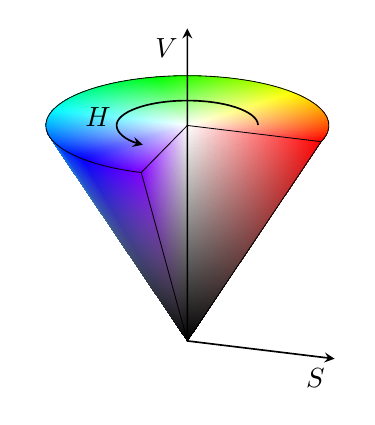
\begin{tikzpicture}[
        >=stealth,
    ]
            \def\arcbegin{0}
            \def\arcending{270}
        \begin{axis}[
            view={19}{30},
            axis lines=center,
            axis on top,
            domain=0:1,
            y domain=\arcbegin:\arcending,
            xmin=-1.5, xmax=1.5,
            ymin=-1.5, ymax=1.5,
            zmin=0.0, zmax=1.2,
            hide axis,
            samples=20,
            data cs=polar,
            mesh/color input=explicit mathparse,
            shader=interp,
        ]
            % -----------------------------------------------------------------
            % also added the "color parts"
            % -----------------------------------------------------------------
            % cone:
            \addplot3 [
                surf,
                variable=\u,
                variable y=\v,
                point meta={symbolic={Hsb=v,u,u}},
            ] (v,u,u);
            % top plane:
            \addplot3 [
                surf,
                samples=50,
                variable=\u,
                variable y=\v,
                point meta={symbolic={Hsb=v,u,1}},
            ] (v,u,1);
            % slice plane
            \addplot3 [
                surf,
                variable=\u,
                y domain=0:1,
                variable y=\w,
                point meta={symbolic={Hsb=\arcbegin,u,z}},
            ] (\arcbegin,u,{u+w*(1-u)});
            \addplot3 [
                surf,
                variable=\u,
                y domain=0:1,
                variable y=\w,
                point meta={symbolic={Hsb=\arcending,u,z}},
            ] (\arcending,u,{u+w*(1-u)});
            % -----------------------------------------------------------------
            % border
            \addplot3 [
                line width=0.3pt,
            ] coordinates {
                (0,0,0) (\arcbegin,1,1) (0,0,1)
                ({(\arcending)},1,1) (0,0,0)
            };
            %%%%%%% border top
            \draw [line width = 0.3pt]
                (axis cs: {cos(\arcbegin)}, {sin(\arcbegin)},1)
%                arc (\arcbegin:\arcending:100)             % <-- old version
                arc (\arcbegin:\arcending:1)                % <-- new version
            ;
            %%%%%%% arc
            \draw [->,line width = 0.6pt]
                (axis cs: {0.5*cos(\arcbegin+20)}, {0.5*sin(\arcbegin+20)},1)
%                arc ({\arcbegin+20}:{\arcending-20}:50)    % <-- old version
                arc ({\arcbegin+20}:{\arcending-20}:0.5)    % <-- new version
            ;
            % x and z axis
            \addplot3[
                <->, %% <------------  added this
                line width=0.6pt,
            ] coordinates {
                (\arcbegin,1.1,0)
                (0,0,0)
                (0,0,1.45)
            };
            % annotations
            \node at (axis cs:1.1,0,0)      [anchor=north east] {$S$};
            \node at (axis cs:0,0,1.45)     [anchor=north east] {$V$};
            \node at (axis cs:-.5,0.0,1.0)  [anchor=east]       {$H$};

        \end{axis}
    \end{tikzpicture}
\end{document}